% ****** Start of file aipsamp.tex ******
%
%   This file is part of the AIP files in the AIP distribution for REVTeX 4.
%   Version 4.1 of REVTeX, October 2009
%
%   Copyright (c) 2009 American Institute of Physics.
%
%   See the AIP README file for restrictions and more information.
%
% TeX'ing this file requires that you have AMS-LaTeX 2.0 installed
% as well as the rest of the prerequisites for REVTeX 4.1
%
% It also requires running BibTeX. The commands are as follows:
%
%  1)  latex  aipsamp
%  2)  bibtex aipsamp
%  3)  latex  aipsamp
%  4)  latex  aipsamp
%
% Use this file as a source of example code for your aip document.
% Use the file aiptemplate.tex as a template for your document.
\documentclass[%
 aip,
 jmp,%
 amsmath,amssymb,
%preprint,%
 reprint,%
%author-year,%
%author-numerical,%
]{revtex4-1}

\usepackage{graphicx}% Include figure files
\usepackage{dcolumn}% Align table columns on decimal point
\usepackage{bm}% bold math
%\usepackage[mathlines]{lineno}% Enable numbering of text and display math
%\linenumbers\relax % Commence numbering lines
\usepackage{enumitem}


\begin{document}

%\preprint{AIP/123-QED}

\title[STAT7055 - INTRODUCTORY STATISTICS FOR BUSINESS AND FINANCE]{EXAM CHEAT SHEET (PART I)}% Force line breaks with \\


% \author{A. Author}
%  \altaffiliation[Also at ]{Physics Department, XYZ University.}%Lines break automatically or can be forced with \\
% \author{B. Author}%
%  \email{Second.Author@institution.edu.}
% \affiliation{ 
% Authors' institution and/or address%\\This line break forced with \textbackslash\textbackslash
% }%

% \author{C. Author}
%  \homepage{http://www.Second.institution.edu/~Charlie.Author.}
% \affiliation{%
% Second institution and/or address%\\This line break forced% with \\
% }%

% \date{\today}% It is always \today, today,
%              %  but any date may be explicitly specified

% \begin{abstract}
% An article usually includes an abstract, a concise summary of the work
% covered at length in the main body of the article. It is used for
% secondary publications and for information retrieval purposes. 
% %
% Valid PACS numbers may be entered using the \verb+\pacs{#1}+ command.
% \end{abstract}

% \pacs{Valid PACS appear here}% PACS, the Physics and Astronomy
%                              % Classification Scheme.
% \keywords{Suggested keywords}%Use showkeys class option if keyword
%                               %display desired
\maketitle

% \begin{quotation}
% The ``lead paragraph'' is encapsulated with the \LaTeX\ 
% \verb+quotation+ environment and is formatted as a single paragraph before the first section heading. 
% (The \verb+quotation+ environment reverts to its usual meaning after the first sectioning command.) 
% Note that numbered references are allowed in the lead paragraph.
% %
% The lead paragraph will only be found in an article being prepared for the journal \textit{Chaos}.
% \end{quotation}

\section{Descriptive Statistics}

\begin{itemize}[label={}]
\item Categorical Data: Nominal or Ordinal 
\item Numerical Data: Continuous or Discrete 
\item Quartile: Q1 (25\%), Q2 (50\%), Q3 (75\%)
\item Percentile: Location of $p$-th percentile: $$L_p = (n+1)\frac{p}{100}$$
\item Inter-Quartile Range (IQR): $$IQR = Q_3 - Q_1$$
\item Population Mean: $\mu = \dfrac{1}{N}\sum_{i=1}^{N}X_i$
\item Sample Mean: $\bar{X} = \dfrac{1}{n}\sum_{i=1}^{n}X_i$
\item Population Variance: $$\sigma^2 = \frac{1}{N}\sum_{i=1}^{N}(X_i-\mu)^2 = E(X^2)-(E(X))^2$$ 
\item Sample Variance: 
    \begin{align*}
        s^2 &= \frac{1}{n-1}\sum_{i=1}^{n}(X_i-\bar{X})^2 \\
            &= \frac{1}{n-1}\left( \left(\sum_{i=1}^{n}X_i^2\right) 
             - \frac{\left(\sum_{i=1}^n X_i\right)^2}{n} \right)        
    \end{align*}
\item Coefficient of Variance: $CV=\dfrac{\sigma}{\mu}$, or $cv=\dfrac{s}{\bar{X}}$
\item Population Covariance: 
    \begin{align*}
        \sigma_{XY} &= \frac{1}{N}\sum_{i=1}^{N}(X_i-\mu_{X})(Y_i-\mu_{Y})\\ &= E(XY) - E(X)E(Y)
    \end{align*}
\item Sample Covariance: 
    \begin{align*}
        \hspace{0.2in}
        & s_{XY} = \frac{1}{n-1}\sum_{i=1}^{n}(X_i-\bar{X})(Y_i-\bar{Y}) \\
        & = \frac{1}{n-1}\left( \left(\sum_{i=1}^{n}X_iY_i\right) 
          - \frac{\left(\sum_{i=1}^n X_i\right)\left(\sum_{i=1}^n Y_i\right)}{n} \right)
    \end{align*}
\item Population Correlation Coefficient: $\rho_{XY} = \dfrac{\sigma_{XY}}{\sigma_{X}\sigma_{Y}}$
\item Sample Correlation Coefficient: $r_{XY} = \dfrac{s_{XY}}{s_{X}s_{Y}}$
\item Note: $-1 \leq \rho_{XY},\ r_{XY} \leq 1$
\item Skewness:
\begin{itemize}[label={}]
\item Zero Skewness: Symmetric (mean = median)
\item Positively Skewed: Long tail to the \textit{right}
\item Negatively Skewed: Long tail to the \textit{left}
\end{itemize}
\item Boxplots:\\\\
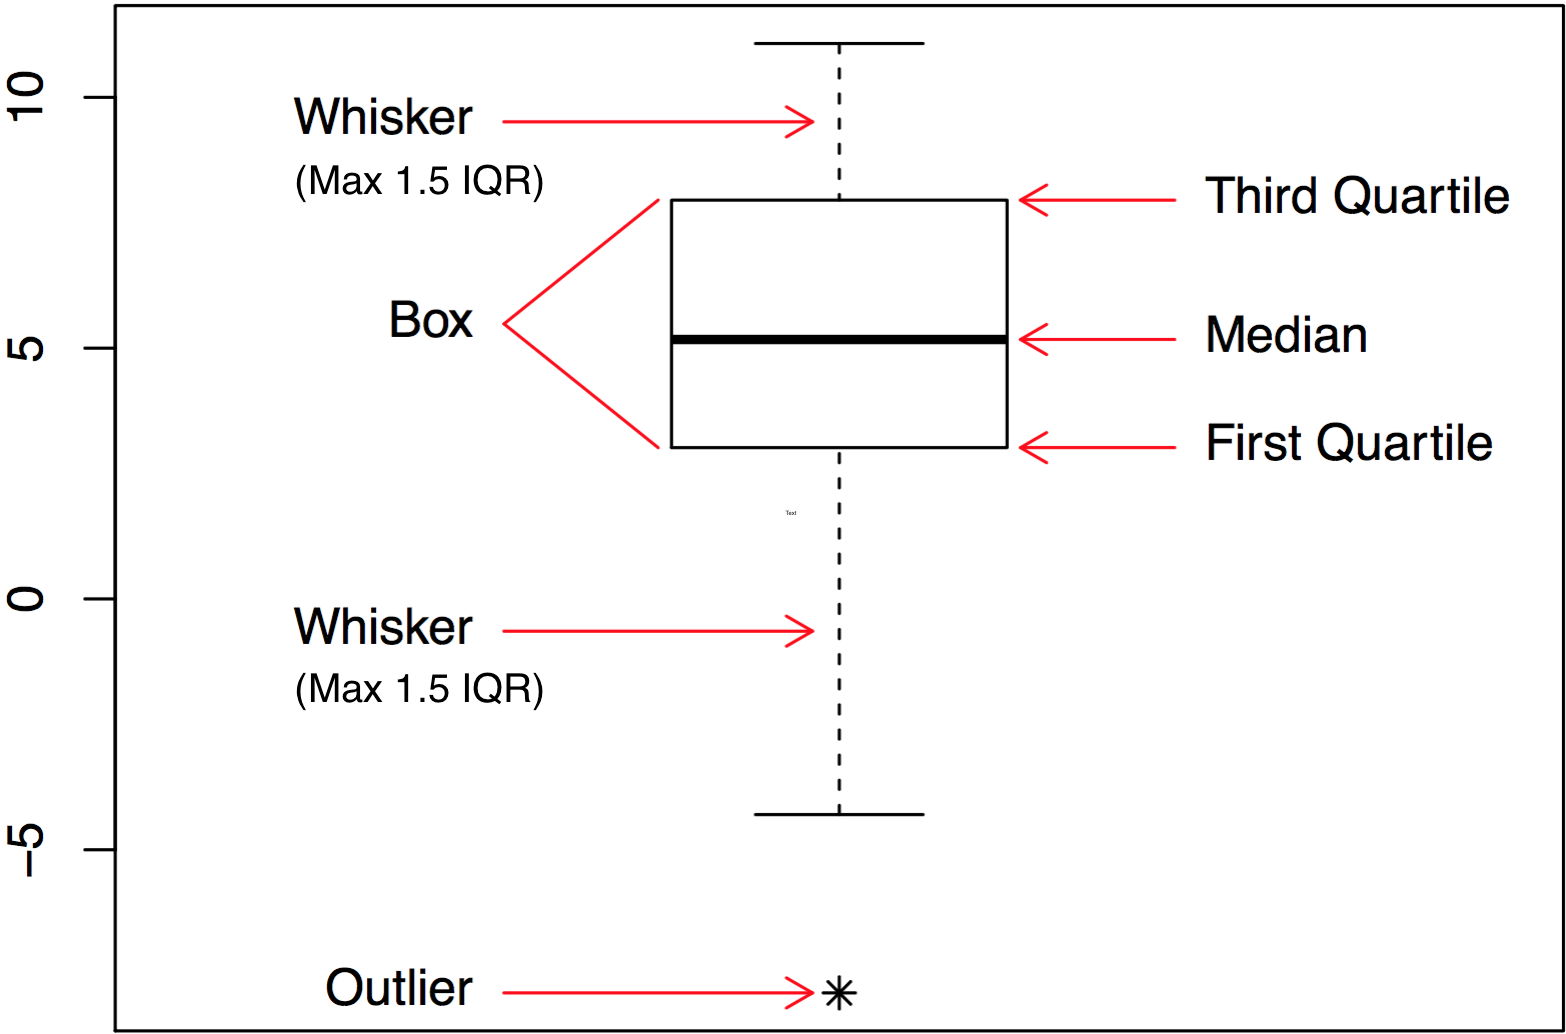
\includegraphics[scale=0.24]{Boxplot}

\end{itemize}

\section{Probability}
\begin{itemize}[label={}]
\item Mutually Exclusive $\Leftrightarrow P(A \cap B) = 0$
\item Independent $\Leftrightarrow P(A \cap B) = P(A)\cdot P(B)$
\item Law of Total Probability: $$ P(A) = \sum_{i=1}^{n} P(A \cap B_i)$$
where $B_1,B_2,\dots, B_n$ are mutually exclusive and $B_1 \cup B_2 \cup \dots \cup B_n = S$ (exhaustive).
\item Multiplication Rule: 
\begin{equation*}
\begin{aligned}
P(A \cap B) &= P(A|B) \cdot P(B) = P(B|A) \cdot P(A)\\
P(A \cap B) &= P(A) \cdot P(B),\ \textrm{if A,B independent}
\end{aligned}
\end{equation*}
\item Addition Rule: 
\begin{equation*}
\begin{aligned}
P(A \cup B) &= P(A) + P(B) - P(A \cap B) \\
P(A \cup B) &= P(A) + P(B), \textrm{if mutually exclusive}
\end{aligned}
\end{equation*}
\item Complement Rule: $P(A^C) = 1 - P(A)$
\end{itemize}

\section{Discrete Probability Distribution}
\begin{itemize}[label={}]
\item Random Variable: $X, Y, Z$
\item Realised Variable: $x, y, z$
\item Expected Value: $\mu = E(X) = \sum_{all\ x}(x \cdot p(x))$
\item Variance: $\sigma^2 = V(X) = E(X^2) - E^2(X)$
\item Joint Probability: $p(x,y)=P(\{X=x\} \cap \{Y=y\})$
\item Marginal Probability: $p_X(x) = \sum_{all\ y}p(x,y)$
\item If $X,Y$ independent: $$p(x,y)=p_X(x)p_Y(y),\ \textrm{for all}\ x,y$$
\item $E(c)=c$, $E(cX)=cE(X)$
\item If $X,Y$ independent: $E(XY) = E(X)E(Y)$
\item $V(c)=0$, $V(X+c)=V(X)$, $V(cX)=c^2V(X)$
\item $E(aX+bY) = aE(X) + bE(Y)$
\item $V(aX+bY) = a^2V(X) + b^2V(Y) + 2abCov(X,Y)$
\item Covariance: $Cov(X,Y)= E(XY) - E(X)E(Y)$
\item Independent $\Rightarrow Cov(X,Y)=0$

\item Binomial Distribution: $X \sim Bin(n,p)$
\item $P(X=x) = \dbinom{n}{x}p^x(1-p)^{n-x}$
\item $E(X)=np,\ V(X)=np(1-p)$
\item Binomial Table: Value is $P(X \leq k)$
\end{itemize}

\section{Continuous Probability Distribution}
\begin{itemize}[label={}]
\item Probability Density Function (PDF): $f(x)$
\item $P(a<X<b) = \int_{a}^{b}f(x)dx$
\item Expected Value: $$ \mu = E(X) = \int_{-\infty}^{\infty}xf(x)dx $$
\item Variance: 
\begin{equation*}\begin{aligned}
\sigma^2 = V(X) &= \int_{-\infty}^{\infty}(x-\mu)^2f(x)dx \\
&= \Big( \int_{-\infty}^{\infty}x^2f(x)dx \Big) - \mu^2
\end{aligned}\end{equation*}
\item Uniform Distribution: $X \sim U(a, b)$
\item $f(x) = \dfrac{1}{b-a}$, $a\leq x \leq b$
\item $E(X) = \dfrac{a+b}{2}$, $V(X) = \dfrac{(b-a)^2}{12}$
\item Normal Distribution: $X \sim N(\mu, \sigma^2)$
$$ f(x) = \frac{1}{\sigma\sqrt{2\pi}}e^{-\frac{(x-\mu)^2}{2\sigma^2}},\ -\infty < x < \infty $$
\vspace{0.01in}
\item $E(X) = \mu$, $V(X) = \sigma^2$
\item Standard Normal Distribution: $$Z = \frac{X-\mu}{\sigma} \sim N(0,1)$$
\item $z$-table: Value is $P(Z < z)$ 
\item $z$-values frequently used: \\
$|z_{0.1}|=1.282$, $|z_{0.05}|=1.645$, $|z_{0.025}|=1.96$, $|z_{0.01}|=2.327$, $|z_{0.005}|=2.576$, $|z_{0.001}|=3.091$
\end{itemize}

\section{Sampling Distribution}
\begin{itemize}[label={}]
\item Mean of $\bar{X}$: $\mu_{\bar{X}}=\mu$
\item Variance of $\bar{X}$ (Standard Error): $\sigma_{\bar{X}}^2 = \dfrac{\sigma^2}{n}$
\item Central Limit Theorem:
$$\bar{X} \sim N(\mu_{\bar{X}}=\mu, \sigma_{\bar{X}}^2=\frac{\sigma^2}{n}),\ \textrm{as}\ x \rightarrow \infty $$
\item Sample Proportion (of Bernoulli trials): $\hat{p}=\frac{X}{n}$
$$\hat{p} \sim N \left(\mu_{\hat{p}}=p, \sigma_{\hat{p}}^2=\frac{p(1-p)}{n} \right)$$
\end{itemize}

\section{Estimation}
\begin{itemize}[label={}]
\item Point Estimator \& Interval Estimator
\item Bias: $B(\hat{\theta})=E(\hat{\theta}) - \theta$. Unbiased if $B(\hat{\theta})=0$
\item Mean Squared Error(MSE): $$MSE(\hat{\theta})=E((\hat{\theta}-\theta)^2)=V(\hat{\theta})+B^2(\hat{\theta})$$
\item $\hat{\theta}$ is consistent if $MSE(\hat{\theta})\rightarrow 0$ as $n \rightarrow \infty$
\item Relative Efficiency: $\textrm{eff}(\hat{\theta_1}, \hat{\theta_2})=\dfrac{V(\hat{\theta_2})}{V(\hat{\theta_1})}$
\item $\hat{\theta_1}$ is better if $\textrm{eff}>1$; $\hat{\theta_2}$ is better if $\textrm{eff}<1$
\item Confidence Interval of $100(1-\alpha)\%$: $\bar{X} \pm z_{\frac{\alpha}{2}}\dfrac{\sigma}{\sqrt{n}}$
\item Lower confidence limit; Upper confidence limit; Cofidence level
\item Interpretation: In repeated sampling, $100(1-\alpha)\%$ of such intervals created would contain the true population mean.\\
\end{itemize}


\end{document}
%
% ****** End of file aipsamp.tex ******
